\chapter{Au boulot~!}

Nous allons maintenant entrer dans le vif du sujet~: la réflexion autour de la structure du projet et son implantation.

\helpbox{Note}{ne consultez cette partie que si vous ne savez plus quoi faire.

\par Avant de la consulter, appelez un assistant à la rescousse, il pourra vous donner des astuces.

\par Chacune des sections suivantes vous donneront des astuces des plus générales aux plus fines. Lisez les en fonction de votre besoin.}

\helpbox[rouge]{NB}{Les solutions proposées ici ne sont que des propositions. Il y a bien évidemment des solutions (dont certaines pourraient être meilleures), n'oubliez pas que vous êtes libres~!}

\section{Lister les classes nécessaires}

Commencez par regarder une capture d'écran du jeu et essayez de repérez les différents objets ou éléments~:

\begin{figure}[!hb]
  \begin{center}
    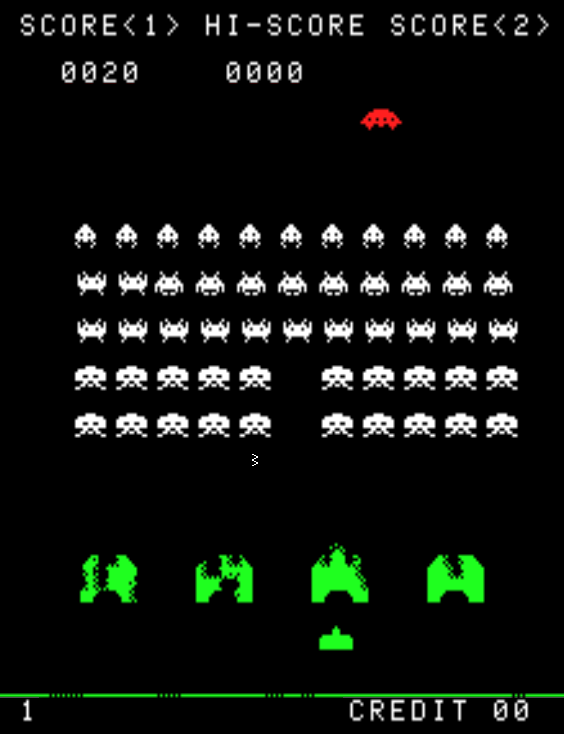
\includegraphics[scale=0.462]{images/space_game1.png}
  \end{center}
\end{figure}

Voilà ce que vous devriez trouver~:

\begin{figure}[!h]
  \begin{center}
    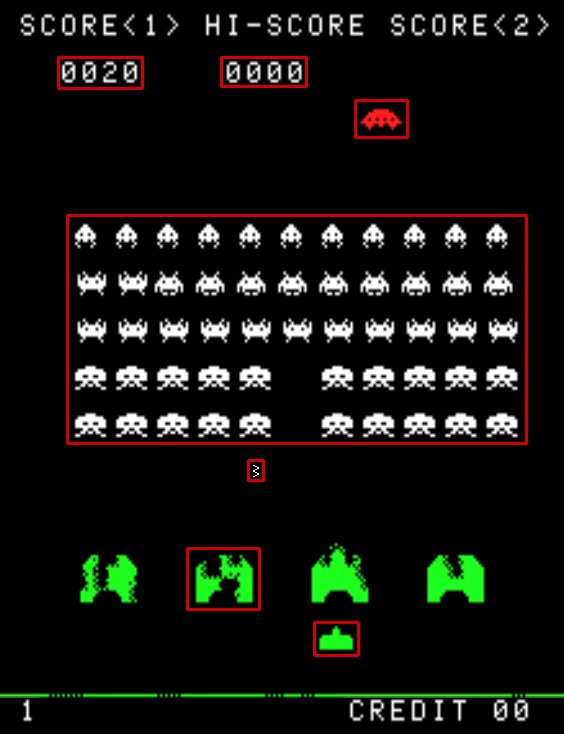
\includegraphics[scale=0.462]{images/space_game12.png}
  \end{center}
\end{figure}

Nous pouvons déjà regrouper certains objets~: les monstres et les soucoupes ont les mêmes caractéristiques. Les projectiles ascendant ou descendant sont aussi à regrouper.\\

Nous nous retrouvons donc avec les classes suivantes~:
\begin{itemize}
   \item \textbf{Monstre~:} représentant les poulpes, les crabes, les séches et les soucoupes.
   \item \textbf{Bouclier~:} empêche les projectiles de passer.
   \item \textbf{Projectile~:} ascendant ou descendant.
   \item \textbf{Joueur~:} vaisseau du joueur, \ldots
\end{itemize}

La classe \texttt{General} fait office de \emph{core engine}, elle servira à stocker les différentes instances des classes ainsi que tout ce qui ne fait parti d'aucune classe~: les scores, \ldots


\section{Quid du moteur graphique~?}

Vous avez un membre du groupe qui ne fait rien sous prétexte que la surcouche implante déjà le moteur graphique du jeu~? C'est pas aussi simple que cela.

Profitez de la boucle d'affichage \texttt{Draw} pour voir comment vous pourriez afficher un monstre, puis deux, etc.

Une fois ceci fait, n'oubliez pas que les sprites des monstres changent de manière régulière~!


\section{Que mettre dans les classes~?}

Replongez-vous une nouvelle fois dans le jeu et prennez chaque classe une par une.\\

Posez-vous les bonnes questions~: d'où vient le courant, par où passe-t-il, qu'est-ce que je cherche~?\footnote{Petite dédicace à notre cher professeur d'électronique, M. {\textsc Gabon}, pour ses questions pertinentes qui changent la vie.} En l'occurence, il n'y a pas de courant (qui a dit qu'il fallait l'imaginer \ldots?), mais que cherchez-vous concrètement~?

\subsection{La classe des monstres}

Très bien, alors que peuvent faire les monstres~?

\begin{itemize}
  \item \textbf{Ils sont distincts~:} chaque monstre a un type propre (un sprite différent entre les poulpes, les crabes et les seiches~; la soucoupe a en plus un déplacement particulier).
  \item \textbf{Ils bougent~:} il faut prévoir quelque chose pour qu'ils se déplacent, savoir où ils sont dans l'espace, vers où ils se déplacent.
  \item \textbf{Ils font gagner des points~:} c'est d'ailleurs étroitement lié à leur type\ldots
  \item \textbf{Ils peuvent être mort~:} si l'on veut afficher l'image d'explosion par exemple. Un petit quelque chose pour savoir s'il est touché peut être pratique.
  \item \textbf{Ils peuvent attaquer~:} envoyer des projectiles. Peut-être que cela serait plus adapté de faire cela dans la classe générale.
\end{itemize}

\subsection{La classe des boucliers}

En régigeant ce \tp, nous n'avons pas trouvé de manière simple de gérer les boucliers~; dans un premier temps, allez au plus simple en arrêtant tous les projectiles qui les touchent.

À partir de là, leur seul point intéressant est leur position.

\subsection{La classe des projectiles}

Que font les projectiles~?

Tout comme les monstres, ils sont \textbf{distincts} (ascendant ou descendant et des sprites différents), ont une position sur l'écran et se déplacent.

\subsection{La classe du joueur}

Le joueur représente le vaisseau en bas de l'écran. Il faut donc savoir où il se trouve, savoir le nombre de vies qu'il lui reste. Il peut également se faire toucher par des projectiles.

\subsection{La classe principale}

Elle doit stocker les données du jeu en cours. Si l'on regarde l'écran de jeu, on peut facilement faire une petite liste.\\

Que diriez-vous d'une petite liste de monstres~? Un joueur (1 dans un premier temps, puis deux~!), sans oublier cette liste de projectiles. Et pour finir un tableau de boucliers. En bonus, pourquoi pas ajouter quelques variables comme un état de pause, de menu, le nombre de pièces insérées, \ldots

Une méthode pour générer le jeu vous permettra de recommencer la partie si le joueur tue tous les monstres. N'oubliez pas d'initialiser ailleurs les autres variables~!

\helpbox{Note}{une liste est différente d'un tableau~! Une liste est dynamique alors qu'un tableau a une taille statique. Suivant votre implantation des monstres, une liste peut être plus adaptée. Elle est cependant nécessaire pour les projectiles.}

Il ne faut pas oublier d'envoyer des soucoupes de temps en temps~!


\section{Mettre à jour les données et les afficher}

\subsection{Les boucles de jeu}

Vous avez à votre disposition, dans la classe principale (\texttt{General}) deux boucles de jeu~: \texttt{Update} qui s'occupe de mettre à jour l'ensemble des données (faire bouger les monstres, faire avancer les projectiles, \ldots) et \texttt{Draw} qui se charge exclusivement de lire les données pour envoyer les objets à la surcouche.\\

Si vous regardez le premier argument passé à ces deux méthodes, il s'agit d'un intervalle de temps (\texttt{TimeStamp}). Il s'agit du temps qu'il s'est écoulé depuis le dernier appel à \texttt{Update} et respectivement \texttt{Draw}

\helpbox[vert]{Information complémentaire}{les deux boucles de jeu n'ont pas forcément le même intervalle de mise à jour. La boucle de jeu \texttt{Update} tentera de s'éxécuter le plus souvent possible, tandis que la boucle d'affichage sera appelée moins souvent afin d'être sur que le jeu s'éxécute normalement malgrès un affichage plus découpé.\\\emph{Space Invaders} est un jeu tout simple, vous ne verrez donc pas la différence, cela se ressent plus lorsque le jeu est beaucoup plus complexe et que les machines sont encore moins performantes~!}

\subsection{Mise à jour des données}

Parcourez votre liste de projectiles, une méthode \texttt{move} permettrait de les déplacer en fonction du temps écoulé depuis le dernier update. Puisqu'il est dans la nature du projectile de tuer, il peut être pratique de profiter du mouvement pour tester les collisions avec les monstres et/ou le joueur. Vous pouvez faire cela dans la même méthode ou dans une méthode séparée. Vous devrez dans les deux cas passer à votre fonction la liste de monstres et de joueur(s).\\

Utilisez l'événement \texttt{OnKeyDown} pour détecter l'appuie sur une touche fléche gauche (\texttt{Left}) ou fléche droite (\texttt{Right}). Il ne sera déclenché qu'une seule fois, pensez à sauvegarder l'état de chaque touche dans une variable que vous replacerez à sa valeur initiale lorsque l'événement \texttt{OnKeyUp} correspondant à une touche que vous attendez est déclenché.

De la même manière que vous déplacez les projectiles, une méthode pourrait permettre au vaisseau du joueur de se déplacer en fonction du temps écoulé et de la direction correspondant à la touche appuyée (et que faire lorsque les deux touches sont enfoncées~?).\\

N'oubliez pas qu'il est rare de voir un joueur avoir des vies négatives~! Et que le jeu recommence (sans effacer le score) lorsqu'il n'y a plus de monstres à tuer~!

\subsection{Affichage des sprites}

Un parcours de la liste des monstres paraît indiqué.

N'oubliez pas qu'à chaque appel de la boucle d'affichage, les éléments que vous aviez envoyé à la surcouche sont effacés. À chaque appel vous devez donc renvoyer l'ensemble des textes et textures.\\

Si vous ne savez pas comment afficher une texture, consultez la liste des méthodes graphiques utiles de la section \ref{ssec:methodutiles} page \pageref{ssec:methodutiles}.\\

Une fois que vous avez les monstres affichés sur l'écran, il ne vous sera pas plus difficile d'afficher le vaisseau du joueur, les boucliers ainsi que les projectiles.

N'oubliez pas les chaînes de caractères présentes en haut de l'écran que vous afficherez sans peine grâce à la méthode \texttt{addString}.


\section{Encore plus de précisions~?}

\subsection{Que faire lorsque l'on a plus de vie~?}

Dans un premier temps, vous pouvez simplement quitter le jeu en utilisant la méthode \texttt{quit} dans l'instance \texttt{action}.

\subsection[Autres précisions]{Vous ne trouvez pas de réponse à votre question~?}

Appelez un assistant qui attend avec enthousiasme de répondre à votre question.\\

Consultez la page d'accueil de votre serveur. Si beaucoup de questions sont répétés, il est possible que ce document soit édité et qu'une mise à jour soit publiée, peut-être que vous trouverez la réponse à votre question.